\section{Multi-Agent Graph-CoT Framework}\label{sec:framework}

\begin{figure}[t]
    \centerline{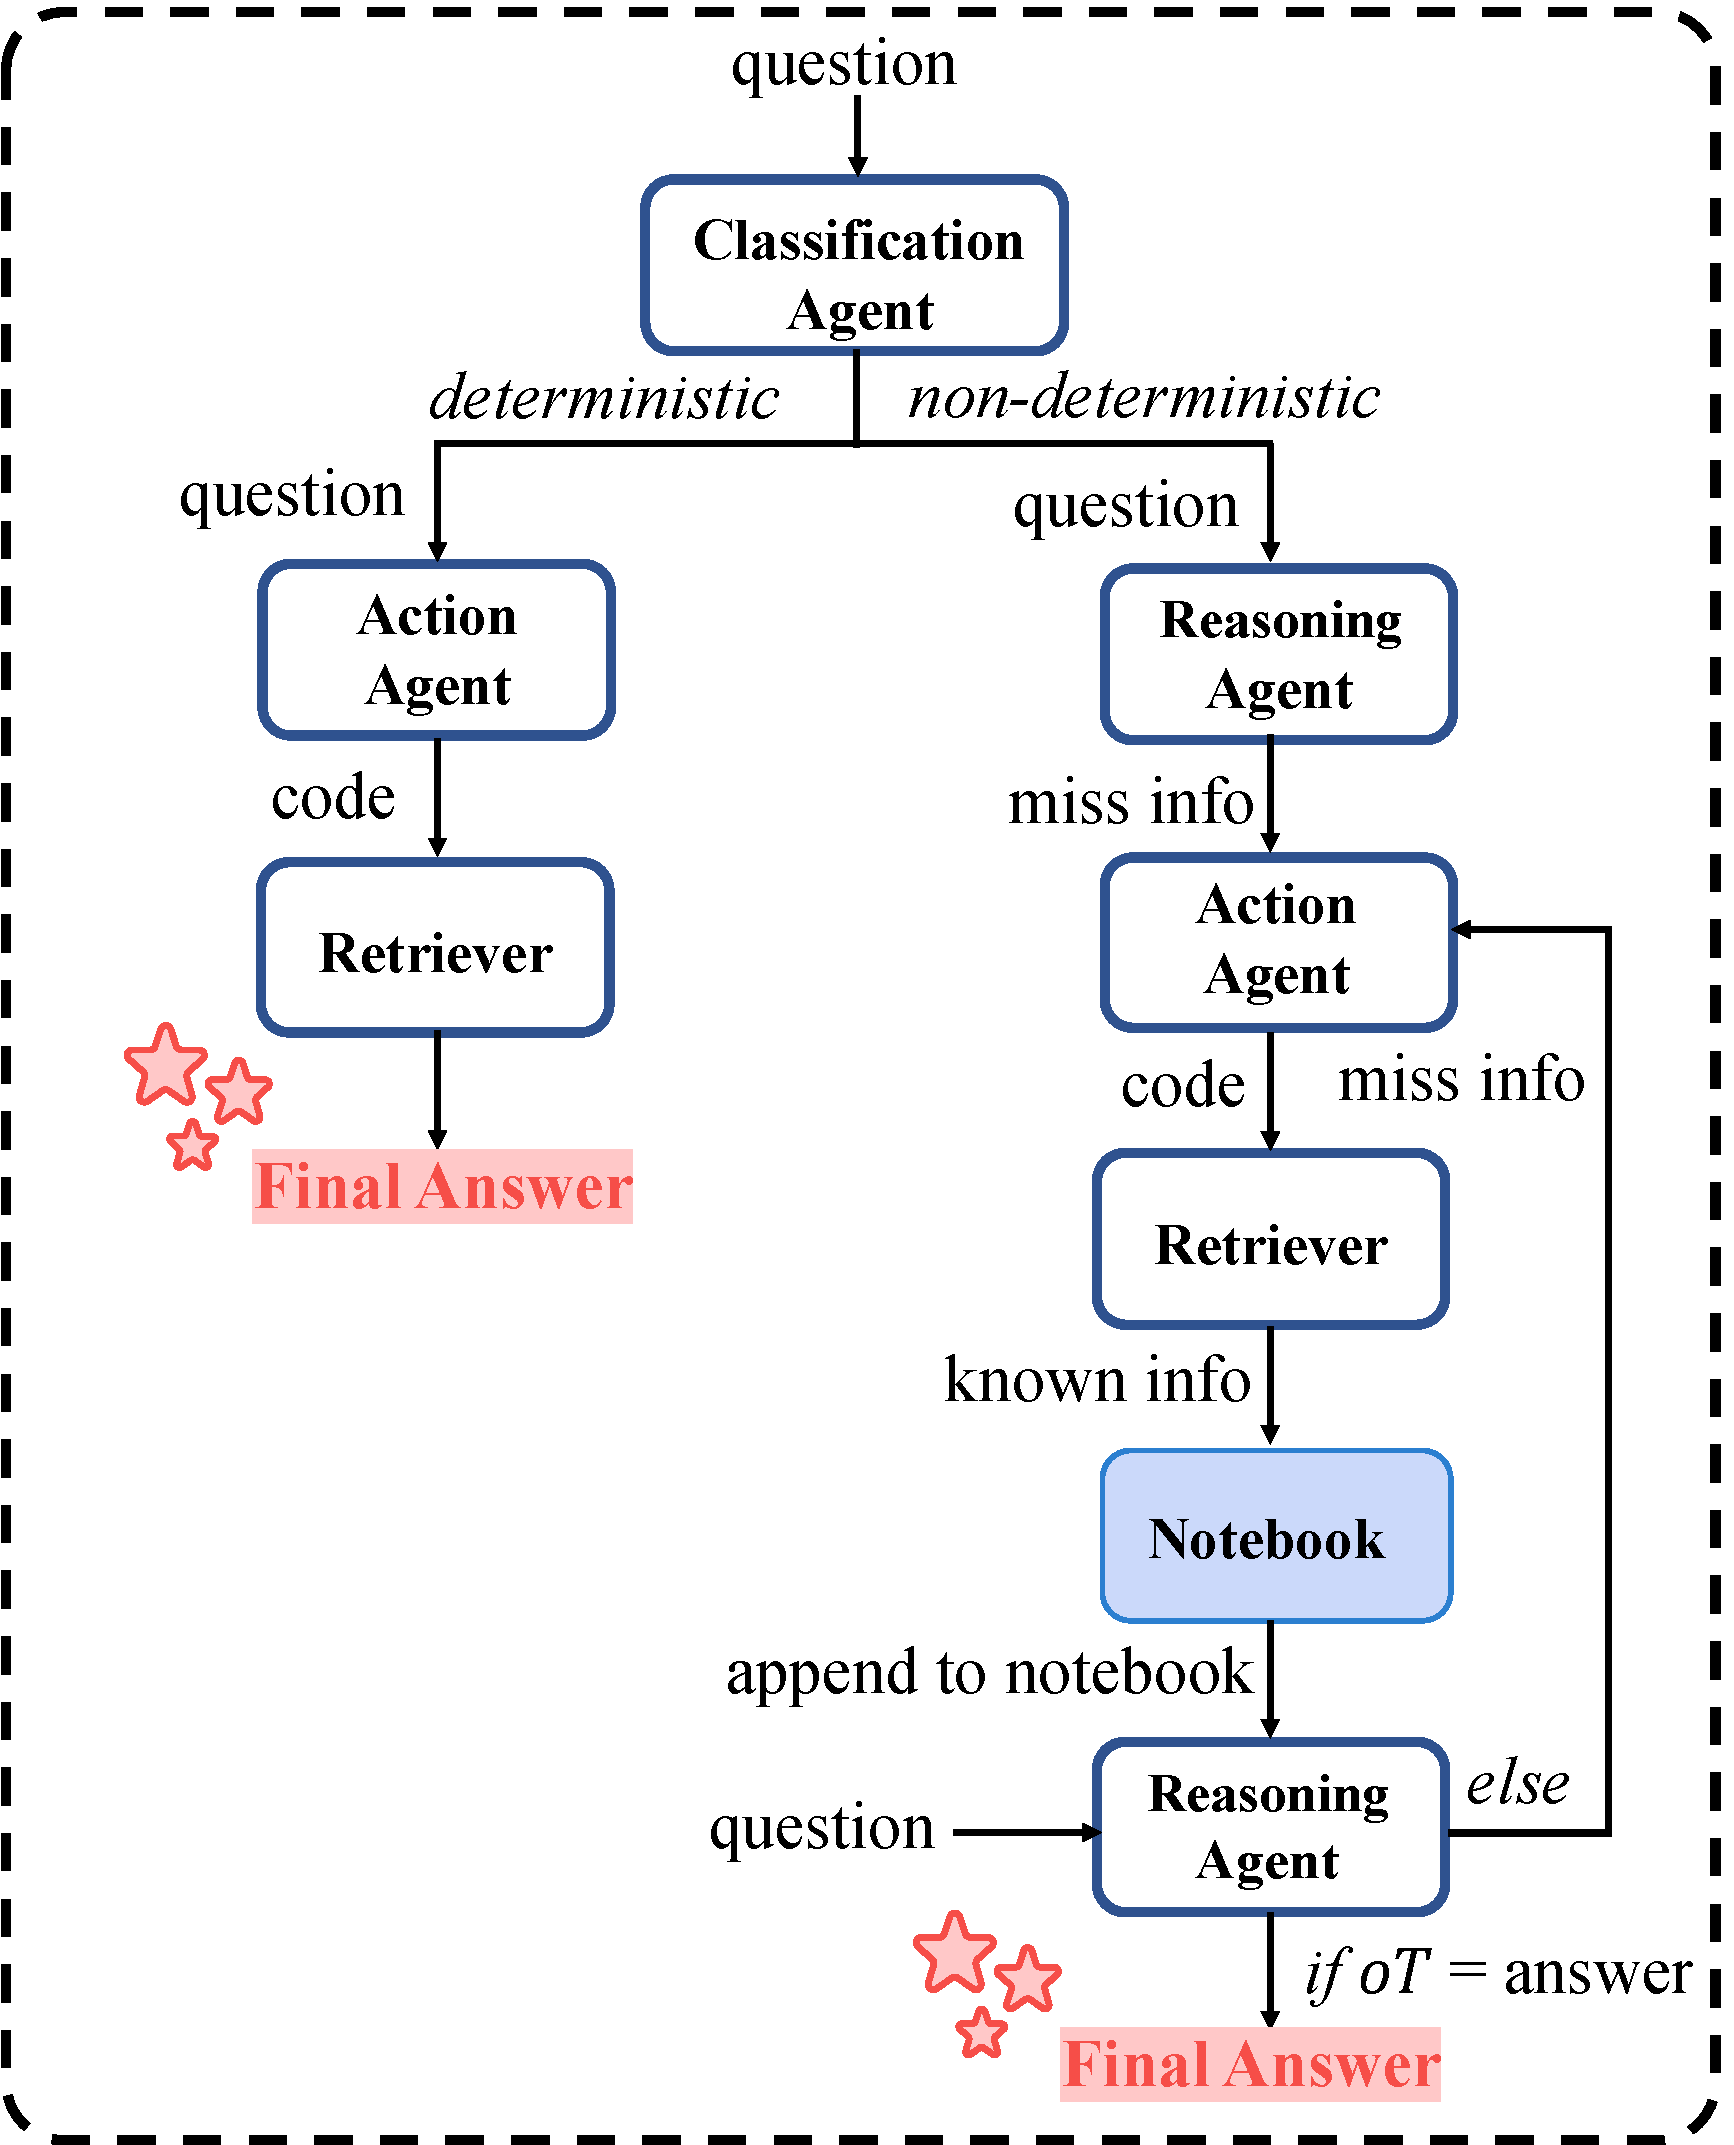
\includegraphics[width=.8\linewidth]{figures/system_overview.pdf}}
    \caption{Multi-agent reasoning framework workflow.}
    \label{fig:system_overview}
\end{figure}


% an efficient multi-agent-based Graph-CoT (Chain-of-Thought) LLM inference collaboration framework
%\subsection{Multi-Agent Reasoning Framework}
\subsection{Overview}
We first introduce \projectname's multi-agent Graph-CoT framework, designed to improve accuracy while reducing token usage (Figure~\ref{fig:system_overview}). It comprises a Graph RAG retriever and three LLM agents: a classifier (C-Agent), a reasoner (R-Agent), and an action generator (A-Agent). Agents operate on task-specific inputs and invoke the inference engine to produce intermediate or final outputs, while the retriever supplies the necessary graph facts at each step. We next formalize the LLM-agent abstraction.

% \begin{definition}[\textbf{LLM-based Agent}]
% Given a large language model (LLM) service defined as:
% \[
% LLM: \text{Prompt} \rightarrow \text{Output}
% \]
% an LLM-based agent is defined as a 3-tuple:
% \[
% \text{X Agent} = (I_x, P_x, O_x)
% \]
% where:
% \begin{itemize}[leftmargin=*, wide, itemindent=0pt]
%     \item $I_x$ denotes the input space of $\text{X Agent}$, comprising outputs from upstream agents, user queries, or graph information.
%     \item $P_x$ represents the prompt template used by $\text{X Agent}$, which takes $I_x$ as input parameters and translates them into instructions for the LLM—guiding it to complete specific tasks such as logical reasoning, summarization, or code generation.
%     \item $O_x$ denotes the output space of $\text{X Agent}$, comprising all possible outputs it may produce upon completion of its task.
% \end{itemize}
% \end{definition}

\begin{definition}[\textbf{LLM-based Agent}]
Given an LLM service defined as: $LLM: \text{Prompt} \rightarrow \text{Output}$, an LLM-based agent is a 3-tuple, $\text{X-Agent} = (I_x, P_x, O_x)$, where $I_x$ is the input space (e.g., outputs from upstream agents, user queries, or graph information), $P_x$ is the prompt template that maps $I_x$ to LLM instructions (enabling tasks such as reasoning, summarization, or code generation), and $O_x$ is the output space comprising all possible outputs of LLM. The execution mechanism of an agent involves applying its agent-specific prompt template \( P_x \) to a given input \( i \in I_x \), generating a formatted prompt that is then passed to the LLM to produce the final output $ o \in O_x $. Formally, this can be expressed as: $o = \text{LLM}(P_x(i)).$
\end{definition}

Building on the agent definition above, we now introduce the specific agents used in our multi-agent reasoning framework, as illustrated in Figure~\ref{fig:agent_prompt}.


\begin{figure}[t]
    \centerline{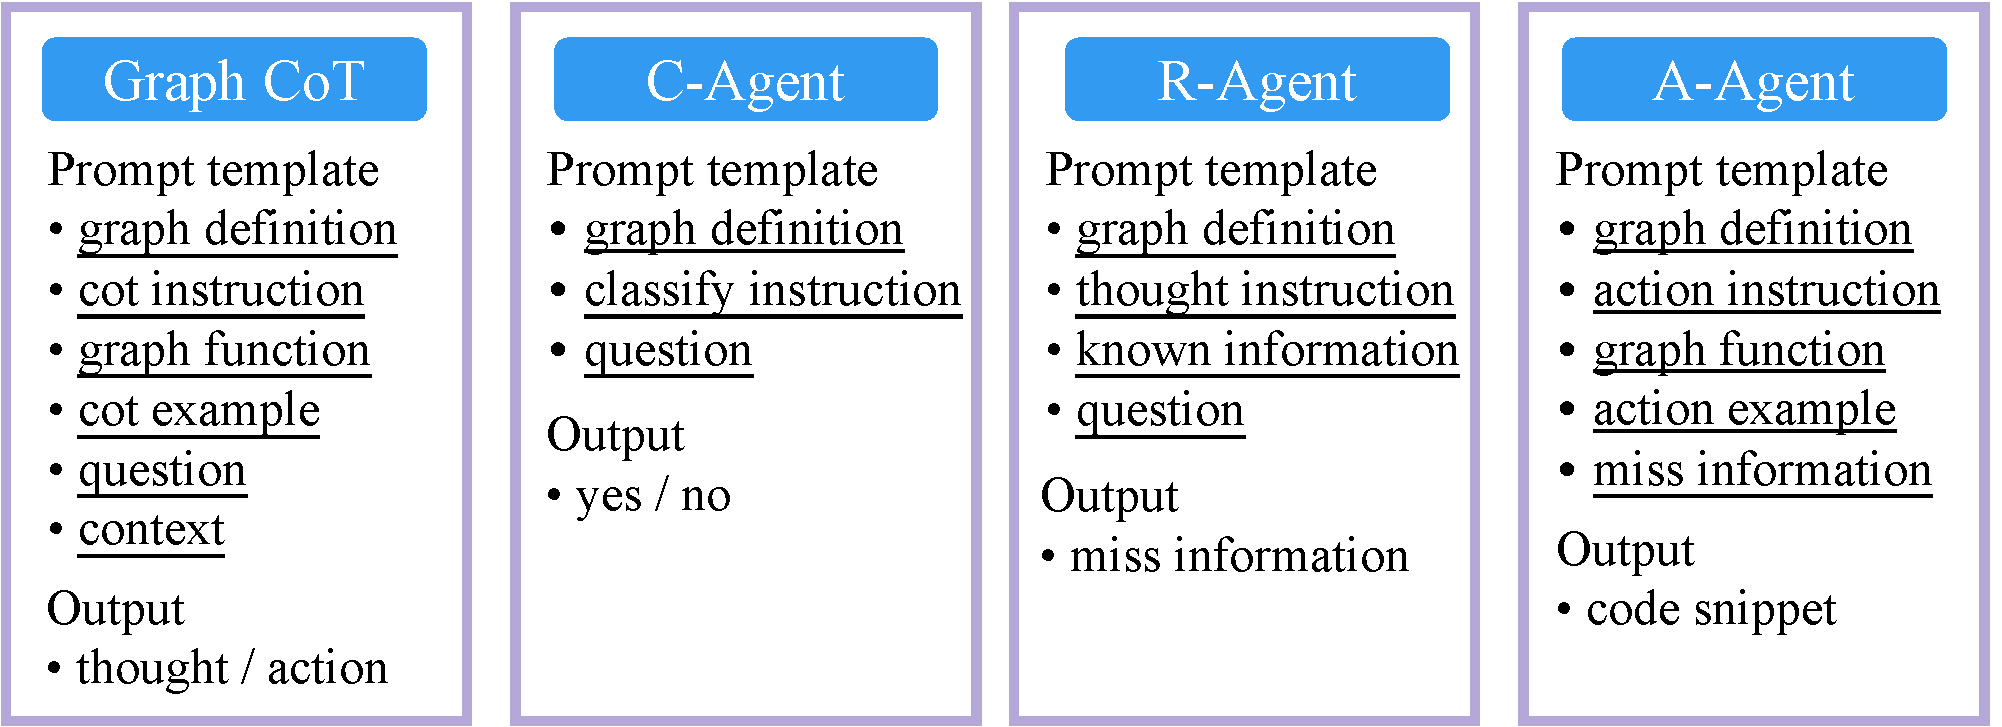
\includegraphics[width=1\linewidth]{figures/agent_prompt.pdf}}
    \caption{Graph-CoT and GLM's agents comparison.}
    \label{fig:agent_prompt}
\end{figure}
%As shown in Figure~\ref{fig:agent_prompt}, our framework comprises three LLM-based agents, each responsible for a distinct reasoning task, and a Graph RAG retriever that supports knowledge-grounded prompt augmentation.


\textbf{Classification Agent (C-Agent).}
The \textit{Classification Agent} determines whether a question is \textit{deterministic} or \textit{non-deterministic}. Deterministic questions can be answered directly by retrieving information from the graph, such as “What is the price of A?”. Non-deterministic questions, like “Recommend the next item based on user history: A, B,” require multi-hop reasoning over multiple nodes and relationships.  

Formally, \(\text{C-Agent}=(I_c,P_c,O_c)\), where \(I_c\) is the natural-language question, \(P_c\) is the prompt template for classification, and \(O_c\in\{\text{deterministic},\text{non-deterministic}\}\).

%Decides whether a question is \emph{deterministic} (answerable by direct retrieval and  computation from the graph; e.g., “price of A”) or \emph{non-deterministic} (requires multi-hop reasoning; e.g., “recommend the next item given history A,B”). 
%Formally, \(\text{C-Agent}=(I_c,P_c,O_c)\), where \(I_c\) is the natural-language question, \(P_c\) is the prompt template for classification, and \(O_c\in\{\text{deterministic},\text{non-deterministic}\}\).

\textbf{Reasoning Agent (R-Agent).}
The \textit{Reasoning Agent} is responsible for determining whether the currently known information is sufficient to answer a given question. If the available information is insufficient, the agent identifies what additional information is required. Otherwise, it proceeds to provide the final answer directly. The \textit{Reasoning Agent} operates through a \textit{notebook} mechanism, which accumulates and maintains known facts during the chain-of-thought reasoning process. At each step, the notebook is updated with new facts retrieved from the graph by the retriever.

Formally, the Reasoning Agent is defined as:
$
\text{R-agent} = (I_t, P_t, O_t),
$
where $I_t$ is the input space, consisting of the current notebook (i.e., known facts) and the user question; \( P_t \) is the prompt template, which encodes this information to guide reasoning; and \( O_t \) is the output space, representing either the final answer or a specification of additional information needed.

\iffalse
\textbf{Classification Agent.}
The primary role of the \textit{Classification Agent} is to determine whether a given question is \textit{deterministic} or \textit{non-deterministic}. A deterministic question can be answered directly by retrieving and computing information from the graph. For example, the query "What is the price of A?" can be resolved by simply accessing the price attribute of node A. In contrast, a non-deterministic question requires reasoning that goes beyond a direct graph lookup. For instance, the query "Recommend the next item based on user history: A, B" requires inference over multiple nodes and their relationships, making it unsuitable for resolution through simple retrieval.

Formally, the Classification Agent is defined as:
$
\text{C-Agent} = (I_c, P_c, O_c),
$
where $I_c$ is the input space, representing the natural language question; \( P_c \) is the prompt template, which formats the input question to guide the LLM in performing classification; and \( O_c \) is the output space, consisting of binary labels: ``yes'' (deterministic) or ``no'' (non-deterministic).


\textbf{Reasoning Agent.}
The \textit{Reasoning Agent} is responsible for determining whether the currently known information is sufficient to answer a given question. If the available information is insufficient, the agent identifies what additional information is required. Otherwise, it proceeds to provide the final answer directly. The \textit{Reasoning Agent} operates through a \textit{notebook} mechanism, which accumulates and maintains known facts during the chain-of-thought reasoning process. At each step, the notebook is updated with new facts retrieved from the graph by the retriever.

Formally, the Reasoning Agent is defined as:
$
\text{R-agent} = (I_t, P_t, O_t),
$
where $I_t$ is the input space, consisting of the current notebook (i.e., known facts) and the user question; \( P_t \) is the prompt template, which encodes this information to guide reasoning; and \( O_t \) is the output space, representing either the final answer or a specification of additional information needed.
\fi




\textbf{Action Agent (A-Agent).}
The \textit{Action Agent} generates executable Python code snippets to retrieve the missing information identified by the \textit{Reasoning Agent}. Unlike prior Graph-CoT systems~\cite{jin2024graph}, which limit actions to predefined operations, our agent produces expressive code that can combine multiple functions, use basic control structures (e.g., \texttt{if-else}, \texttt{for}), and employ standard data types (\texttt{set}, \texttt{list}, \texttt{dict}). This allows complex reasoning to be completed in a single execution step, reducing multi-round interactions. The agent outputs only the essential results via \texttt{print()}, avoiding redundant intermediate context.


Formally, the \textit{Action Agent} is defined as:
$
\text{A-Agent} = (I_a, P_a, O_a),
$
where $I_a$ is the input space, representing the missing information specified by the \textit{Reasoning Agent}; \( P_a \) is the prompt template, which encodes the task of generating the corresponding code snippet; and \( O_a \) is the output space, consisting of the generated Python code.

\begin{algorithm} [t]
\caption{Multi-Agent Reasoning Workflow.}
\label{alg:workflow}
\small
\begin{algorithmic}[1]
\Require Question $q$, $\text{C-Agent}$, $\text{R-agent}$, $\text{A-Agent}$, Retriever, LLM service.
\State $o_c \gets LLM(P_c(q))$
\If{$o_c ==$ \text{yes}}
    \State $o_a \gets LLM(P_a(q))$
    \State $a \gets Retriever(o_a)$
\Else
    \State Initialize notebook $n \gets \{\}$
    \While{$True$}
        \State $o_t \gets LLM(P_t(n, q))$
        \If{$o_t$ indicates answer completeness}
            \State $a \gets o_t$
            \State \textbf{break}
        \Else
            \State $o_a \gets LLM(P_a(o_t)))$
            \State $o_r \gets Retriever(o_a)$
            \State $n \gets n \cup \{o_r\}$
        \EndIf
    \EndWhile
\EndIf
\State \Return final answer $a$
\end{algorithmic}
\end{algorithm}

\textbf{Graph RAG Retriever.}
In addition to the LLM-based agents, a key component of \projectname is the \textit{Graph RAG Retriever}, which bridges the \textit{Action Agent} and the underlying graph. When the \textit{Action Agent} generates a Python snippet to obtain missing information, it is executed via Python’s \texttt{exec()} function, and the results are appended to the agent’s notebook as new knowledge for subsequent reasoning. We build upon the Graph-CoT~\cite{jin2024graph} retrieval interface and extend it with a new function, \texttt{NodeInfo()}, which provides vertex-centric contextual information (see Section~\ref{sec:vertex_centric_kv}). Specifically, \texttt{RetrieveNode()} maps entities to node IDs through vector search over the graph’s embedding index (GPU-accelerated), while other functions map node IDs to their attributes and metadata stored in an in-memory dictionary. Table~\ref{tab:function_summary} summarizes all core functions, including our extensions.


\iffalse


\textbf{Graph RAG Retriever.}
In addition to the LLM-based agents, a key component of the framework is the \textbf{Graph RAG Retriever}, which facilitates interaction between the \textit{Action Agent} and the underlying graph database. After the \textit{Action Agent} generates a Python code snippet to retrieve missing information, the snippet is executed using Python’s \texttt{exec()} function. The resulting outputs are treated as newly acquired knowledge and appended to the agent’s notebook, thereby supporting subsequent reasoning steps.  

We adopt the same graph retrieval interface as Graph-CoT~\cite{jin2024graph} and extend it by introducing an additional function, \texttt{NodeInfo()}, which provides vertex-centric contextual information (see Section~\ref{sec:vertex_centric_kv}). Specifically, the \texttt{RetrieveNode()} function establishes the mapping between entities and node IDs by performing a vector search over the graph’s embedding index, which can be accelerated on GPUs. The remaining functions handle mappings from node IDs to their corresponding metadata and attributes, which are efficiently retrieved from an in-memory dictionary constructed from the graph. The core functions, including our extensions, are summarized in Table~\ref{tab:function_summary}.
\fi

\begin{table*}[ht]
\centering
\small
\begin{tabular}{|l|l|l|l|}
\hline
\textbf{Function} & \textbf{Input} & \textbf{Output} & \textbf{Function Description} \\
\hline
RetrieveNode & text & nodeID & Returns the ID of the node most relevant to the input text using vector similarity. \\
\hline
NodeInfo & nodeIDs & vertex chunk & Returns the vertex chunk for the given node. \\
\hline
NodeFeature & nodeIDs, featureName & values & Retrieves feature values for the given nodes. \\
 % If no feature name is given, returns all features.
\hline
NodeDegree & nodeID, neighbourType & degree & Returns the number of neighbours of the specified type for the given node. \\
\hline
neighbourCheck & nodeID, neighbourType & nodeIDs & Returns the neighbours of the specified type for the given node. \\
\hline
\end{tabular}
\caption{Summary of core graph-related functions in Graph RAG retriever.}
\label{tab:function_summary}
\end{table*}


\subsection{Workflow}
Upon receiving a question $q$, \projectname initiates a multi-agent reasoning workflow, coordinating interactions between LLM-based agents and the Graph RAG retriever, as detailed below:

\noindent \textbf{Step 1:} The \textit{Classification Agent} determines whether $q$ is deterministic or non-deterministic. If $q$ is deterministic, we proceed directly to Step~3. Otherwise, we move to Step~2.

\noindent \textbf{Step 2:} For non-deterministic questions, the \textit{Action Agent} generates a code snippet $o_a$ based on $q$. This snippet is executed by the \textit{Graph RAG retriever} to obtain relevant information from the graph dataset. The final answer is then extracted and returned using the \texttt{print} statement within the executed code.

\noindent \textbf{Step 3:} Initialize an empty notebook $n = \{\}$. The \textit{Reasoning Agent} takes $q$ and $n$ as input and produces the missing information $o_t$.

\noindent \textbf{Step 4:} Enable iterative chain-of-thought reasoning: (1) \textit{Action Agent:} Generate a code snippet $o_a$ from $o_t$; (2) \textit{Graph RAG Retriever:} Execute $o_a$ and append the result to the notebook $n$; (3) \textit{Reasoning Agent:} Generate the next $o_t$ based on $q$ and $n$.

% This iterative process repeats until a termination condition is satisfied (i.e., $o_t$ constitutes a complete answer), after which $o_t$ is returned as the final output. The overall workflow is detailed in Algorithm~\ref{alg:workflow}.

This iterative process continues until a termination condition is met, whereby the output of \textit{Reasoning Agent} $o_t$ represents a complete answer to the original query. At that point, $o_t$ is returned as the final output of the system. The overall workflow is detailed in Algorithm~\ref{alg:workflow}.

%The entire reasoning process is formally outlined in Algorithm~\ref{alg:workflow}, which summarizes the interactions described above.

% \begin{algorithm} [ht]
% \caption{Multi-Agent Reasoning Workflow}
% \label{alg:workflow}
% \begin{algorithmic}[1]
% \Require Question $q$, $\text{C-Agent}$, $\text{R-agent}$, $\text{A-Agent}$, Retriever, LLM service.
% \State Initialize notebook $n \gets \{\}$
% \State $result \gets LLM(P_c(q))$
% \If{$result ==$ \text{yes}}
%     \State $code\_snippet \gets LLM(P_a(q))$
%     \State $answer \gets Retriever(code\_snippet)$
% \Else
%     \While{$True$}
%         \State $thought \gets LLM(P_t(n, q))$
%         \If{$thought$ is the final answer}
%             \State $answer \gets thought$
%         \Else
%             \State $code\_snippet \gets LLM(P_a(o_t)))$
%             \State $known\_info \gets Retriever(o_a)$
%             \State $n \gets n \cup \{known\_info\}$
%         \EndIf
%     \EndWhile
% \EndIf
% \State \Return final answer $a$
% \end{algorithmic}
% \end{algorithm}


% \textbf{Workflow.} Once we receive a question, it will forward it to our \projectname's multi-agent LLM system, which is composed of multiple specialized agents, each responsible for a distinct function but collaborate together by engaging in chain-of-thought reasoning. During this process, the LLM system interacts dynamically with the Graph RAG component to retrieve and integrate relevant structured knowledge. Graph RAG serves as an external knowledge database for the LLM agents. It provides additional context by allowing the agents to retrieve information through a dedicated retriever module. The LLM system generates appropriate code snippets, which are executed via the retriever to query an index built on a structured graph dataset. The retrieved results are then appended to a notebook, enriching the reasoning process with accurate and relevant information from the graph. This iterative interaction continues until the LLM system converges on a correct and well-supported answer.

% After introducing the overall workflow, we now provide a detailed description of each component in the Multi-Agent framework. As shown in Figure~\ref{fig:agent_prompt}, each agent is designed with a distinct role and input structure, tailored to its specific function. There are four main agents: the Classification Agent, Thought Agent, Action Agent, and Retriever, which we refer to as \textbf{C-Agent}, \textbf{R-agent}, \textbf{A-Agent}, and \textbf{Retriever}, respectively. The process begins with the C-Agent, which determines whether the input question requires step-by-step reasoning. For deterministic questions, the system directly proceeds to the A-Agent. For non-deterministic questions, the R-agent iteratively generates missing information needed to answer the question. The A-Agent then retrieves this missing information through executable actions, and the new knowledge is appended to the known context. This loop continues until the R-agent determines the answer is complete, at which point the final answer is produced.

% \underline{\textit{Large Language Models:}} Once \projectname receives a question, it first forwards it to a multi-agent LLM system. The LLM system is a framework composed of multiple specialized agents, each responsible for a distinct function. These agents collaborate by engaging in chain-of-thought reasoning, where they iteratively reason through multiple steps. During this process, the LLM system interacts dynamically with the Graph RAG component to retrieve and integrate relevant structured knowledge. This iterative interaction continues until the LLM system converges on a correct and well-supported answer.

% \underline{\textit{Graph RAG:}} Graph RAG serves as an external knowledge database for the LLM agents. It provides additional context by allowing the agents to retrieve information through a dedicated retriever module. The LLM system generates appropriate code snippets, which are executed via the retriever to query an index built on a structured graph dataset. The retrieved results are then appended to a notebook, enriching the reasoning process with accurate and relevant information from the graph.

% \underline{\textit{Cache Management:}} Cache Management provides foundational support for both the LLM system and the Graph RAG component. It includes two key components: the Prefix KV Cache and the Retrieve Cache. These are designed to reduce latency for LLM inference and Graph RAG retrieval respectively, by leveraging the framework's characteristics and the structure of the graph-based index. This component will be discussed in detail in section \ref{sec: optimization}.

% \subsection{Framework}
% To address the limitations of existing approaches, we propose \projectname, a novel multi-agent-based Graph-CoT (Chain-of-Thought) framework that improves both the quality of LLM-generated responses and the efficiency of inference.

% \textbf{Classification Agent.} 
% The role of the Classification Agent is to determine whether a given question is deterministic or non-deterministic. We define a deterministic question as one that can be answered by retrieving and computing on the graph, For example, "what is the price of A" is a deterministic question which can be answered by retrieve the "price" feature of node A in Graph RAG. while a non-deterministic question requires additional reasoning beyond the information in the graph. For example, in the question Recommend next item based on user history: A, B", this type of question requires reasoning over multiple nodes' features, which cannot be directly answered through simple graph lookup.

% As discussed in Section~\ref{sec:motivation}, using a unified reasoning framework (e.g., Chain-of-Thought prompting) for both types of questions is inefficient. In particular, applying CoT to deterministic questions introduces unnecessary steps, especially when the required information is abundant or straightforward to access. This leads to increased latency and higher token consumption. To address this, each question is first classified. Each question is first classified. For deterministic questions, to avoid unnecessary steps, we treat the question itself as missing information and let the Action Agent generate the corresponding code snippet to get the answer directly. For non-deterministic questions, since it's not possible to know in advance what information will be needed, we adopt a chain-of-thought strategy, allowing the agent to reason step-by-step and interact with the graph iteratively.

% The Classification Agent is made up of a shared prefix and the input question, and it outputs either "yes" or "no".

% \textbf{Thought Agent.}
% The main role of the Thought Action is to determine whether the current known information is sufficient to answer the question when it has been classified as a non-deterministic problem. If the information is not enough, the model should indicate what additional information is needed. If the information is sufficient, then the correct answer should be directly output.

% The Thought Action mainly consists of a shared prefix, a notebook that records known information, and the current question. For each question, the notebook maintains a growing list of facts accumulated during the chain-of-thought (CoT) reasoning process. After each round, the output from Retriever is appended to this notebook as new known information. This process continues until sufficient information has been gathered to answer the question.

% \textbf{Action Agent.}
% The role of the Action Agent is to generate a Python code snippet that retrieves the missing information identified by the Thought Agent. Unlike Graph-CoT\cite{jin2024graph}, where the action output is limited to predefined graph operations, the Action Agent in \projectname\ produces a complete and executable code snippet that may include multiple predefined functions. This design allows one step of thought and action to generate more information, effectively replacing multiple rounds of reasoning with a single, more comprehensive code execution.

% The prompt for the Action Agent includes a shared prefix and the missing information, where the missing information is directly taken from the input to the Thought Agent.

\begin{figure}[t]
    \centerline{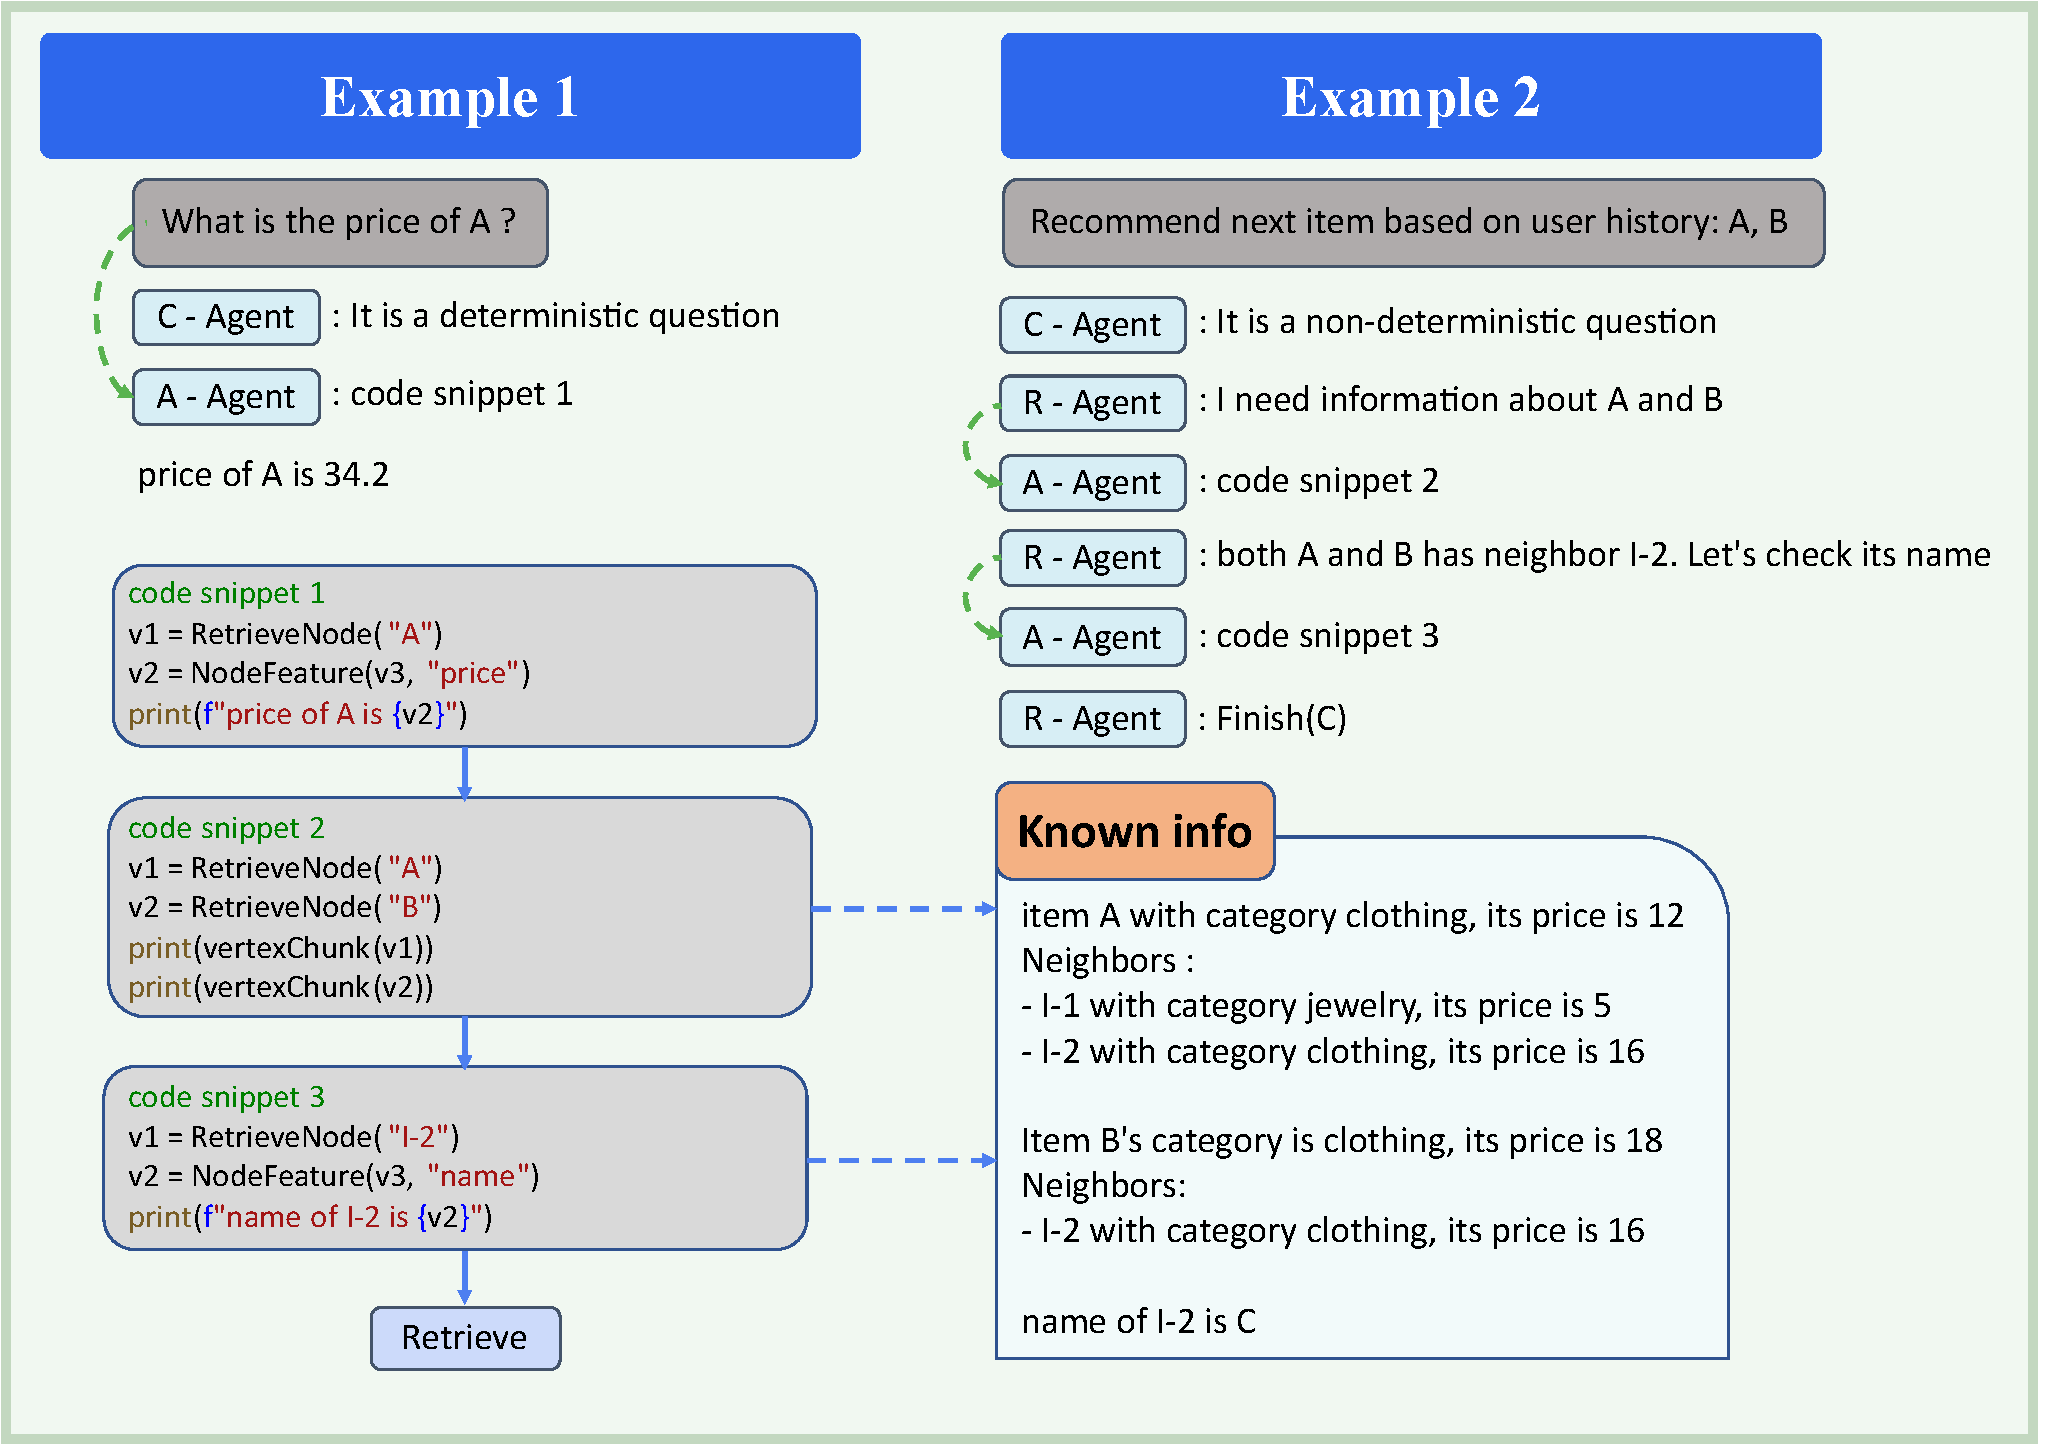
\includegraphics[width=1\linewidth]{figures/framework_example_v1.pdf}}
    \caption{Multi-agent reasoning example.}
    \label{fig:example}
\end{figure}

% \textbf{Case Study.} As illustrated in Figure~\ref{fig:example}, we present two representative examples to demonstrate the workflow of our system. For the question \textit{"What is the price of A?"}, the input is first processed by the C-Agent, which classifies it as a deterministic question. It is then forwarded to the A-Agent with the raw question text as the initial missing information. The A-Agent generates a code snippet and directly prints the final answer. In contrast, for the question \textit{"Recommend next item based on user history: A, B"}, the C-Agent identifies it as a non-deterministic question, then the R-agent first infers what information is missing in order to answer the question. It determines that a complete representation of items \textit{A} and \textit{B} is required. The A-Agent then generates a code snippet to retrieve this information, which is executed by the Retriever and appended to the known context. Based on this updated context, the R-agent observes that both \textit{A} and \textit{B} share a neighbour node \textit{I-2}, and further infers that the name of \textit{I-2} is required. The A-Agent again generates the appropriate code, and the Retriever fetches that node \textit{I-2} corresponds to \textit{Item C}. With all necessary information collected, the R-agent concludes that \textit{Item C} is the appropriate recommendation for the user.

% \textbf{Case Study.} As shown in Figure~\ref{fig:example}, we present two representative examples to illustrate the workflow of our system.
% For the question \textit{"What is the price of A?"}, the input is first handled by the C-Agent, which classifies it as a deterministic question. The question is then passed to the A-Agent with the raw text treated as the initial missing information. The A-Agent generates a code snippet that directly prints the final answer.
% In contrast, consider the question \textit{"Recommend next item based on user history: A, B"}. Here, the C-Agent identifies it as a non-deterministic question. The R-agent first infers what additional information is required to answer the query, determining that full representations of items \textit{A} and \textit{B} are needed. The A-Agent generates a code snippet to retrieve this information, which is executed by the Retriever and appended to the known context. With the updated context, the R-agent observes that both \textit{A} and \textit{B} share a neighbouring item \textit{C}, and its category and price are also similar to those of the items the user has viewed. The R-agent concludes that \textit{Item C} is the most appropriate recommendation for the user.


\textbf{Case Study.}
Figure~\ref{fig:example} shows two flows.
(1) \emph{Deterministic} (“What is the price of A?”): The C-Agent classifies the query as deterministic. The A-Agent produces a one-shot snippet that fetches and prints A’s price. The Retriever executes the snippet and returns the answer.
(2) \emph{Non-deterministic} (“Recommend next item given A,B”): The C-Agent classifies the query as non-deterministic. The R-agent first infers what additional information is required to answer the query, reasoning that full representations of items \textit{A} and \textit{B} are needed. The A-Agent generates a code snippet to retrieve this information, which is executed by the Retriever and appended to the known context. With the updated context, the R-agent observes that both \textit{A} and \textit{B} share item \textit{C}, and its category and price are also similar to those of the items the user has viewed. The R-agent concludes that \textit{Item C} is the most appropriate recommendation for the user.



%\textbf{Case Study.} As shown in Figure~\ref{fig:example}, we present two representative examples to illustrate the workflow of our system.
%For the query \textit{"What is the price of A?"}, the input is first processed by the C-Agent, which classifies it as a deterministic question. The query is then forwarded to the A-Agent, where the raw text is treated as the initial missing information. The A-Agent generates a code snippet that directly retrieves and prints the final answer.
%In contrast, consider the query \textit{"Recommend next item based on user history: A, B"}. Here, the C-Agent classifies it as a non-deterministic question. The R-agent first infers what additional information is required to answer the query, determining that full representations of items \textit{A} and \textit{B} are needed. The A-Agent generates a code snippet to retrieve this information, which is executed by the Retriever and appended to the known context. With the updated context, the R-agent observes that both \textit{A} and \textit{B} share a neighbouring item \textit{C}, and its category and price are also similar to those of the items the user has viewed. The R-agent concludes that \textit{Item C} is the most appropriate recommendation for the user.


% \textbf{Token Usage Analysis.} 
% Let \( T_{\text{G}} \), \( T_{\text{c}} \), \( T_{\text{a}} \), and \( T_{\text{t}} \) denote the average token consumption per invocation by the Graph-CoT framework, the classification agent, the action agent, and the reasoning agent, respectively. We begin with the assumption that the classification agent is lightweight in comparison, such that \( T_{\text{c}} \ll T_{\text{G}} \).

% Under this assumption, we compare the total token consumption of the baseline single-agent Graph-CoT and our proposed framework, \projectname. For Graph-CoT, we assume the reasoning process involves \( k_1 \) steps, each comprising two invocations (e.g., one for generating the next thought and one for selecting the next action). The total token usage is therefore:
% \[
% \text{Tokens}_{\text{Graph-CoT}} = 2k_1 \cdot T_{\text{G}}.
% \]
% In contrast, the token usage of \projectname depends on the nature of the input query. We differentiate between two cases:

% \textbf{Deterministic Questions.} For deterministic questions, \projectname requires only a single invocation of the classification agent and one invocation of the action agent, resulting in total token consumption:
% \[
% \text{Tokens}_{\text{deterministic}} = T_{\text{c}} + T_{\text{a}}.
% \]
% Given that \( T_{\text{c}} \ll T_{\text{G}} \), the overall token cost is substantially lower than that of Graph-CoT.

% \textbf{Non-deterministic Questions.} For non-deterministic questions, \projectname invokes the classification agent once, the action agent \( k_2 \) times, and the reasoning agent \( k_2 + 1 \) times. Based on empirical observation (see Figure~\ref{fig:agent_prompt}), we approximate \( T_{\text{t}} + T_{\text{a}} \approx T_{\text{G}} \). Therefore, the total token consumption can be estimated as:
% \[
% \text{Tokens}_{\text{non-deterministic}} = T_{\text{c}} + k_2 \cdot (T_{\text{t}} + T_{\text{a}}) + T_{\text{t}} 
% \]
% \[
% \approx (k_2 + 1) \cdot T_{\text{G}}.
% \]

% \textbf{Token Reduction.} Compared to Graph-CoT, \projectname achieves notable reductions in token usage. For deterministic questions, the savings are approximately:
% \[
% 2k_1 \cdot T_{\text{G}} - (T_{\text{c}} + T_{\text{a}})
% \]
% \[
% \approx (2k_1 - 1) \cdot T_{\text{G}}.
% \]
% For non-deterministic questions, the savings are:
% \[
% 2k_1 \cdot T_{\text{G}} - (k_2 + 1) \cdot T_{\text{G}} = (2k_1 - k_2 - 1) \cdot T_{\text{G}}.
% \]

% These results highlight the token-efficiency advantages of \projectname across both simple and complex reasoning tasks.

\textbf{Cost Model - Token Usage Analysis.} 
Let \( T_{\text{G}} \), \( T_{\text{c}} \), \( T_{\text{a}} \), and \( T_{\text{t}} \) denote the average token consumption per invocation by the Graph-CoT agent, classification agent, action agent, and reasoning agent, respectively. We assume that \( T_{\text{c}} \ll T_{\text{G}} \). Additionally, as shown in Figure~\ref{fig:agent_prompt}, we approximate that \( T_{\text{a}} + T_{\text{t}} \approx T_{\text{G}} \).

For Graph-CoT, each reasoning step requires two invocations (thought and action), assume that for each question, Graph-CoT requires $k_1$ step, yielding a total of \( 2k_1 \cdot T_{\text{G}} \) tokens.

For \projectname, the token cost depends on the query type. For deterministic queries, only one classification and one action invocation are needed, i.e., \( T_{\text{c}} + T_{\text{a}} \). For non-deterministic queries, the classification agent is called once, while the action agent and reasoning agent are called \( k_2 \) and \( k_2 + 1 \) times, respectively. Based on the assumption, the total becomes approximately \( (k_2 + 1) \cdot T_{\text{G}} \).

As a result, the reduction compared to the baseline Graph-CoT is as follows:  
For deterministic queries, the reduction is approximately \( (2k_1 - 1) \cdot T_{\text{G}} \);  
For non-deterministic queries, the reduction is approximately \( (2k_1 - k_2 - 1) \cdot T_{\text{G}} \).  
These results further highlight the significant token-efficiency advantages of \projectname, demonstrating its superiority across both simple and complex reasoning tasks.

\subsection{Code Generation Optimization} 

% \textbf{Code Generation Definition.}  
Given a graph $g$ and a specification of \emph{missing information} $m$ produced by the Reasoning Agent, \textbf{code generation} defines a mapping $\mathcal{G}: (q, m) \rightarrow s$ that yields an \emph{executable} code snippet $s$.  

\textbf{Code Generation within Graph-CoT.}  
In Graph-CoT, code refers to a predefined set of graph-retrieval functions (\texttt{RetrieveNode}, \texttt{NodeFeature}, \texttt{neighbourCheck}, \texttt{NodeInfo}) that the LLM can invoke to obtain the required information from the graph.  

\textbf{Limitations of Existing Graph-CoT Code Generation.}  
In the original Graph-CoT framework, the LLM interacts with the external graph by selecting from a fixed set of predefined retrieval functions and providing their parameters. This design constrains retrieval granularity and leads to inefficiencies in two common cases. First, when a query requires information from multiple vertices, multiple reasoning rounds must be executed to collect all necessary data. Second, when the target information depends on intermediate computation (e.g., the intersection of two vertices’ neighbour lists), the system must explicitly retrieve and store all intermediate results, increasing both context size and token cost.  

\textbf{Our Approach.} 
To overcome these limitations, we introduce a code generation optimization that enables the Action Agent to synthesize complete executable Python snippets rather than merely selecting from predefined functions. Each snippet is composed only of: (i) the predefined graph-retrieval functions and basic control; (ii) optional \emph{local} computations (e.g., aggregation, set intersection) to derive the precise information required by $m$; and (iii) a minimal \texttt{print()} statement that outputs only the final result, avoiding unnecessary intermediate text. Executing $s$ once against the Graph RAG retriever produces the required facts to update the agent’s notebook or generate the final answer, thereby replacing multiple reasoning rounds with a single deterministic program execution and significantly reducing token usage and latency.  

\textbf{Case Study.}  
As illustrated in Figure~\ref{fig:example_comparison}, for queries requiring information from multiple vertices, a single code snippet can invoke several graph functions within one reasoning round, thereby reducing interaction steps. For queries involving intermediate computations, the snippet performs local data processing (e.g., averaging or intersection) internally, eliminating redundant intermediate storage and minimizing reasoning overhead. This optimization effectively reduces both the number of reasoning rounds and the total token consumption per query.


\begin{figure}
    \centerline{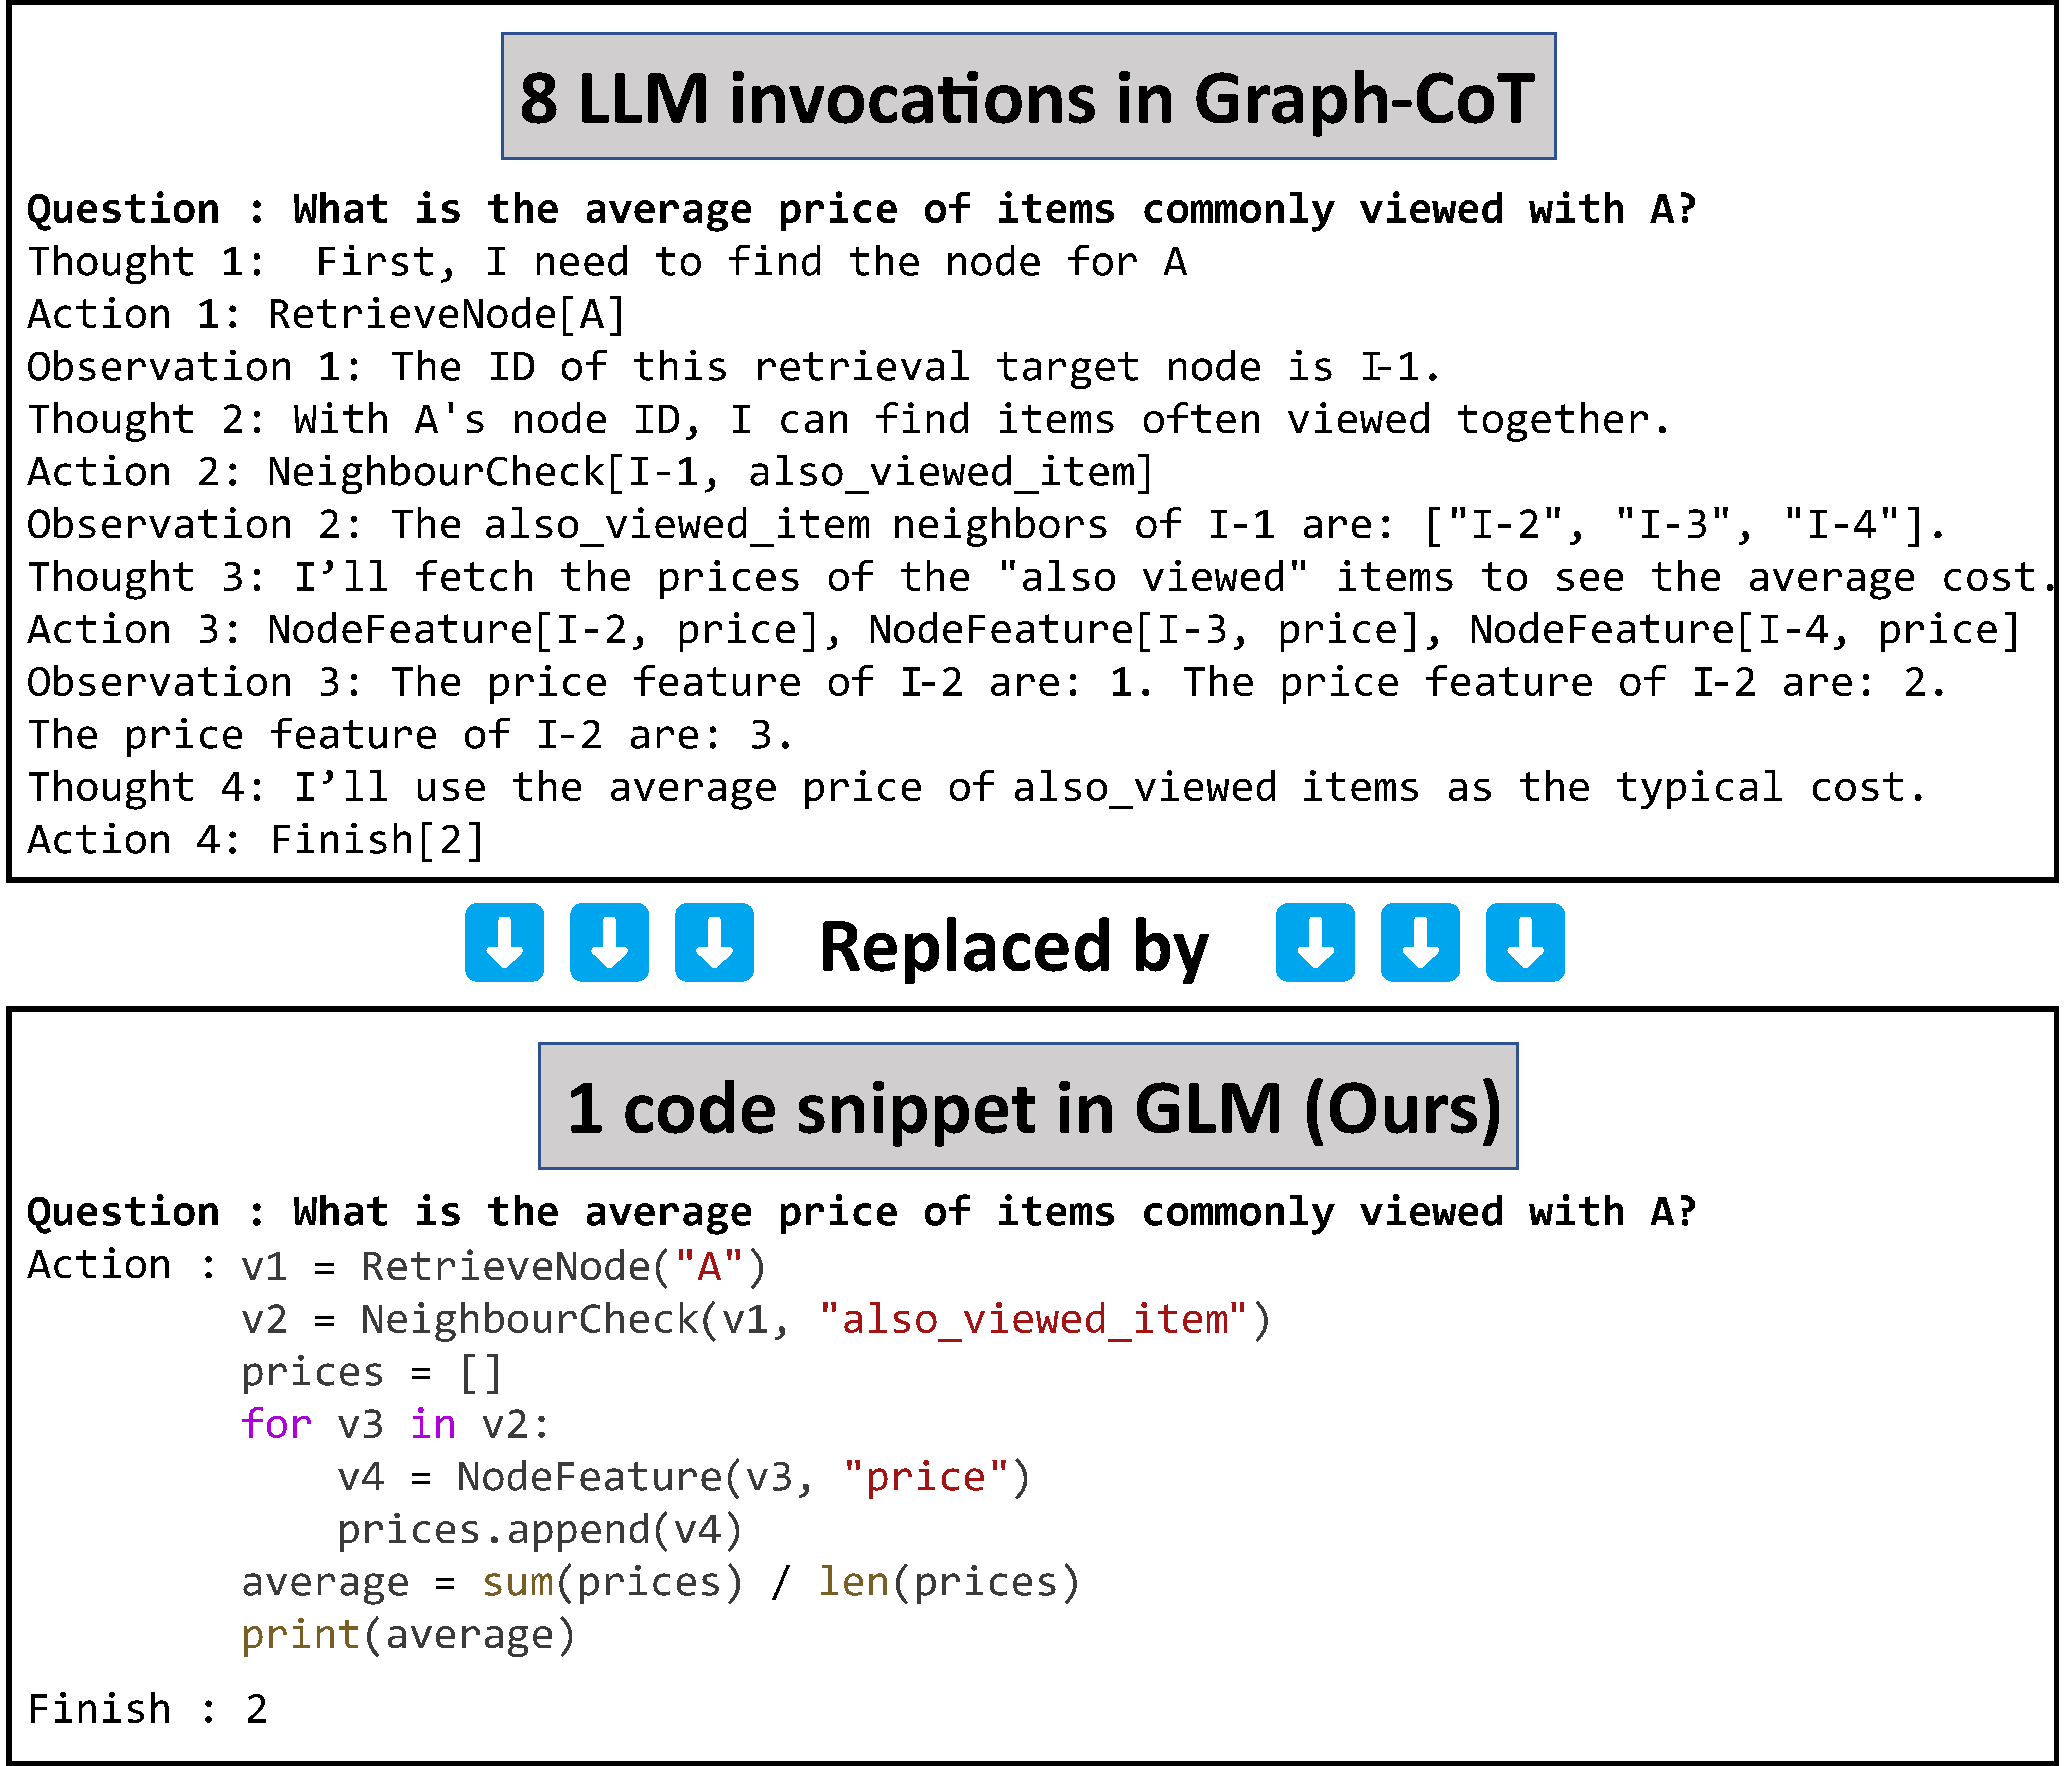
\includegraphics[width=1\linewidth]{figures/background_comparison.pdf}}
    \caption{Code snippet: reducing reasoning steps.}
    \label{fig:example_comparison}
\end{figure}

